\documentclass{article}
\usepackage{custom} %% Have stripped out journal/publisher identifiers and trim marks
% \usepackage{maa-monthly} %% For actual journal style
\usepackage{textcomp}

\usepackage{algorithm2e}

\usepackage{amsfonts}

\theoremstyle{plain}
\newtheorem{theorem}{Theorem}
\newtheorem{lemma}{Lemma}
 
\theoremstyle{definition}
\newtheorem*{definition}{Definition}
\newtheorem*{remark}{Remark}
\newtheorem{example}{Example}

\def \cC {\mathcal{C}}
\def \cG {\mathcal{G}}
\def \cP {\mathcal{P}}
\def \FF {\mathbb{F}}
\newcommand{\AND}{\mathbin{\texttt{\&}}}
\DeclareMathOperator{\im}{im}
\def\And{\mathbin{\&}}
\def\Plus{+}
\DeclareMathOperator{\Span}{span}
\DeclareMathOperator{\Length}{length}

\begin{document}

\title{(Re)constructing code loops}
\markright{Reconstructing code loops}
\author{Ben Nagy and David Michael Roberts}

\maketitle

\begin{abstract}
The Parker loop is a central extension of the extended binary Golay code. It is an example of a general class of non-associative structures known as \emph{code loops}, which have been studied from a number of different algebraic and combinatorial perspectives.
This expository paper aims to also highlight an experimental approach to computing in code loops, by a combination of a small amount of precomputed information and making use of the rich identities that code loops' twisted cocycles satisfy.
As a biproduct one can reconstruct the multiplication in the Parker loop from a mere fragment of its twisted cocycle, and we have found relatively large subspaces of the Golay code over which the Parker loop splits as a direct product.
\end{abstract}


\noindent
The theory of codes makes for a fascinating study. 
At their heart, codes are `merely' subspaces of vector spaces over some small finite field, with certain combinatorial properties.
Why do such things exist? Like a lot of exceptional objects in combinatorics, it can come down to: ``because''.
This makes constructing codes sometimes more of an art than something systematic.
In this paper, we are going to consider the construction of certain structures closely related to codes, called \emph{code loops}. 
We will only consider the case where the base field is $\FF_2=\{0,1\}$, and refer to its elements as \emph{bits}.

The first published example of a code loop appeared as a step in John Conway's construction of the Monster sporadic simple group \cite{Conway}. 
The code loop Conway used originally appeared in an unpublished manuscript by Richard Parker.
A general study of code loops was then made by Robert Griess \cite{Griess}.
Griess also proved the existence of code loops by an algorithmic construction, starting from a particular type of code.
More recent approaches will be discussed below.

Recall that the elements (or \emph{words}) in a code $\cC$, being vectors, can be combined by addition---this is a group operation and hence associative. 
The elements of a code loop consist of a pair: a code word and one extra bit.
The extra bit \emph{twists} the addition so that combination of code loop elements is a \emph{non-associative operation}: $(xy)z\not=x(yz)$ in general.

More specifically, while addition of words in a code is performed by coordinate-wise addition in $\FF_2$ (bitwise XOR) the algebraic operation in a code loop is not so easily described.
The code loop operation can be reconstructed from a function $\cC \times \cC \to \FF_2$ satisfying certain identities, called a \emph{twisted cocycle}.
It is the computation and presentation of these functions that will mainly concern us in this article, using Griess's algorithm \cite[proof of Theorem 10]{Griess}.
As a result, we will observe some curious features of the Parker loop, obtained via experimentation and, it seems, previously unknown.

\section{Extensions and cocycles.}

As a warm-up, we will describe a more familiar structure using the techniques that will be used later. 
Recall that the \emph{quaternion group} $Q_8$ is the group consisting of the positive and negative basis quaternions:
\[
	Q_8 = \{1,\, i,\, j,\, k,\,-1,\, -i,\, -j,\, -k\}
\]
The elements of $Q_8$ satisfy the identities
\[
	i^2 = j^2 = k^2 = -1, \quad ij=k.
\]
There is a surjective group homomorphism $\pi\colon Q_8 \to \FF_2 \times \FF_2 = V_4$, sending $i$ to $(1,0)$ and $j$ to $(0,1)$, and the kernel of $\pi$ is the subgroup $\{1,-1\}\simeq \FF_2$.
Moreover, this kernel is the \emph{center} of $Q_8$, the set of all elements that commute with every other element of the group. This makes $Q_8$ an example of a \emph{central extension}: $\FF_2\to Q_8 \to V_4$.

Now $Q_8$ is a nonabelian group, but both $\FF_2$ and $V_4$ are abelian.
One might think that it shouldn't be possible to reconstruct $Q_8$ from the latter two groups, but it is! 
That is, if we are given some extra information that uses only the two abelian groups.
There is a function $s\colon V_4 \to Q_8$, sending $(0,0)$ to $1$, $(1,0)$ to $i$, $(0,1)$ to $j$ and $(1,1)$ to $k$.
This almost looks like a group homomorphism, but it is not, as $(1,0) + (1,0) = (0,0)$ in $V$, but $s(1,0)s(0,1) = i^2 \not= 1 = s(0,0)$ in $Q_8$.
We can measure the failure of $s$ to be a group homomorphism by considering the two-variable function
\[
	d\colon V_4 \times V_4 \to \FF_2
\]
defined by $ (-1)^{d(v,w)} = s(v)s(w)s(v+w)^{-1}$. 
It is a nice exercise to see that $s(v)s(w)s(v+w)^{-1}$ is always $\pm 1$, so that this definition makes sense. The values of $d(v,w)$ are given as:

\begin{center}
\begin{tabular*}{0.35\textwidth}{c|cccc}
$v\setminus w$&$00$&$10$&$01$&$11$\\
\hline
	$00$		& $0$& $0$& $0$& $0$\\
	$10$		& $0$& $1$& $1$& $0$\\
	$01$		& $0$& $0$& $1$& $1$\\
	$11$		& $0$& $1$& $0$& $1$\\
\end{tabular*}
\end{center}
where $00=(0,0)$, $10=(1,0)$ and so on.
If $s$ \emph{were} a homomorphism, $d$ would be constant at $0$.
One can check that $d$ satisfies the \emph{cocycle identities}:
\[
	d(v,w)-d(u+v,w)+d(u,v+w)-d(u,v) = 0
\]
for all triples $u,v,w\in V_4$. It is also immediate from the definition that $d(0,0)=0$.
An alternative visualisation is given in Figure~\ref{fig:cocycle for q8}.

\begin{figure}[!b]
\begin{center}
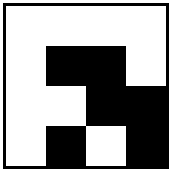
\includegraphics[height=2.5cm]{quaternion_cocyc} %%% Want this to be a pdf image, not png
\end{center}
\caption{A $4\times4$ array giving the values of the cocycle $d\colon V_4\times V_4\to \FF_2$, with white = $0$, black = $1$.}
\label{fig:cocycle for q8}
\end{figure}


The reason for this somewhat mysterious construction is that we can build a bijection of \emph{sets} using $s$ and the isomorphism $\FF_2\simeq \{1,-1\}$, namely
\[
	\FF_2\times V_4 \simeq \left(\{1\}\times V_4\right) \cup \left(\{-1\} \times V_4\right) \stackrel{\phi}{\longrightarrow}
	\{1,\, i,\, j,\, k\}\cup \{-1,\, -i,\, -j,\, -k\} = Q_8\,.
\]
Now, if we define a new product operation on the underlying set of $\FF_2\times V_4$ by
\[
	(s,v)\ast_d(t,w):=(s+ t+ d(v,w),v+w),
\]
then the cocycle identities ensure that this is in fact associative and further, a group operation.
Finally, $\phi$ can be checked to be a homomorphism for the group operation on $Q_8$ and for $\ast_d$, hence is a group isomorphism.

Thus we can reconstruct, at least up to isomorphism, the nonabelian group $Q_8$ from the two abelian groups $V_4$ and $\FF_2$, together with the \emph{cocycle} 
\[
	d\colon V_4\times V_4\to \FF_2.
\]
If we didn't know about the group structure of $Q_8$ already, we could construct it from scratch using $d$.
We can construct the Parker loop using a similar approach.


\section{Twisted cocycles and loops.}

The construction in the previous section is a fairly typical case of reconstructing a central extension from a cocycle (although in general one does not even need the analogue of the group $V_4$ to be abelian). 
However, we wish to go one step further, and construct a structure with a \emph{non-associative} product from a pair of abelian groups: the group $\FF_2$ and additive group of a vector space $V$ over $\FF_2$.
Instead of a cocycle, we use a \emph{twisted cocycle}: a function $\alpha\colon V\times V \to \FF_2$ like $d$ that instead satisfies
\[
	\alpha(v,w)-\alpha(u+v,w)+\alpha(u,v+w)-\alpha(u,v) = f(u,v,w),
\]
for a nonzero \emph{twisting function} $f\colon V\times V\times V \to \FF_2$. We will assume that $\alpha$ satisfies $\alpha(0,v)=\alpha(v,0) = 0$ for all $v\in V$, a property that holds for $d$ in the previous section. From a twisted cocycle the set $\FF_2 \times V$ can be given a binary operation $\ast_\alpha$:
\[
	(s,v)\ast_\alpha(t,w):=(s+ t+ \alpha(v,w),v+w).
\]
We denote $\FF \times V$ equipped with this binary operation by $\FF_2\times_\alpha V$.

Recall that a \emph{loop} is a set $L$ with a binary operation $\star\colon L\times L \to L$, a unit element $e\in L$ such that $e\star x = x \star e = x$ for all $x\in L$, and such that for each $z\in L$, the functions $r_z(x) = x \star z$ and $\ell_z(x)=z\star x$ are bijections $L\to L$. 
Informally, this means that every element $z\in L$ has a left inverse and a right inverse for $\star$, and these are unique---but may be different in general. 
The following is a cute exercise using the twisting function and the assumption that $\alpha(0,v)=\alpha(v,0)=0$.

\begin{lemma}
The operation $\ast_\alpha$ makes $\FF_2\times_\alpha V$ into a loop, with identity element $(0,\underline{0})$, for $\underline{0}$ the zero vector in $V$.
There is a homomorphism $\pi\colon \FF_2\times_\alpha V \to V$ that projects onto the second factor, and whose kernel is $\FF_2 \times\{\underline{0}\}$.
\end{lemma}

Groups are examples of loops, but they are, in a sense, the uninteresting case. 
Arbitrary loops are quite badly behaved: their product is non-associative in general. 
But there is a special non-associative case, introduced by Ruth Moufang \cite{Moufang}, with better algebraic properties.

\begin{definition}
A \emph{Moufang loop} is a loop $(L,\star)$ satisfying the identity
\[
x \star (y \star (x \star z)) = ((x \star y) \star x) \star z
\]
for all choices of elements $x,y,z\in L$.
\end{definition}

The most famous example of a Moufang loop is probably the set of non-zero octonions under multiplication. 
A key property of a Moufang loop $L$ is that any subloop $\langle x,y\rangle < L$ generated by a pair of elements $x,y$ is in fact a group. 
As a corollary, powers of a \emph{single} element are well-defined, and do not require extra bracketing: $x\star (x \star x) = (x\star x) \star x =: x^3$, for example. 
Additionally, the left and right inverses \emph{always} agree in a Moufang loop, so that for each $x\in L$, there is a unique $x^{-1}$ such that $x\star x^{-1} = x^{-1}\star x = e$. 
Importantly for us, code loops, defined below as a special case of the construction of $\FF\times_\alpha V$, turn out to be Moufang.

\begin{example}\label{example:m16}
Let $V= (\FF_2)^3$. The 16-element Moufang loop $M := M_{16}(C_2\times C_4)$ of \cite[Theorem 2]{Chein} is isomorphic to $\FF_2 \times_\mu V$,  arising from a twisted cocycle $\mu\colon V\times V\to\FF_2$ given by the $8\times 8$ array in Figure~\ref{fig:cocycle for M}:
\medskip
\begin{figure}[!hb]
\begin{center}
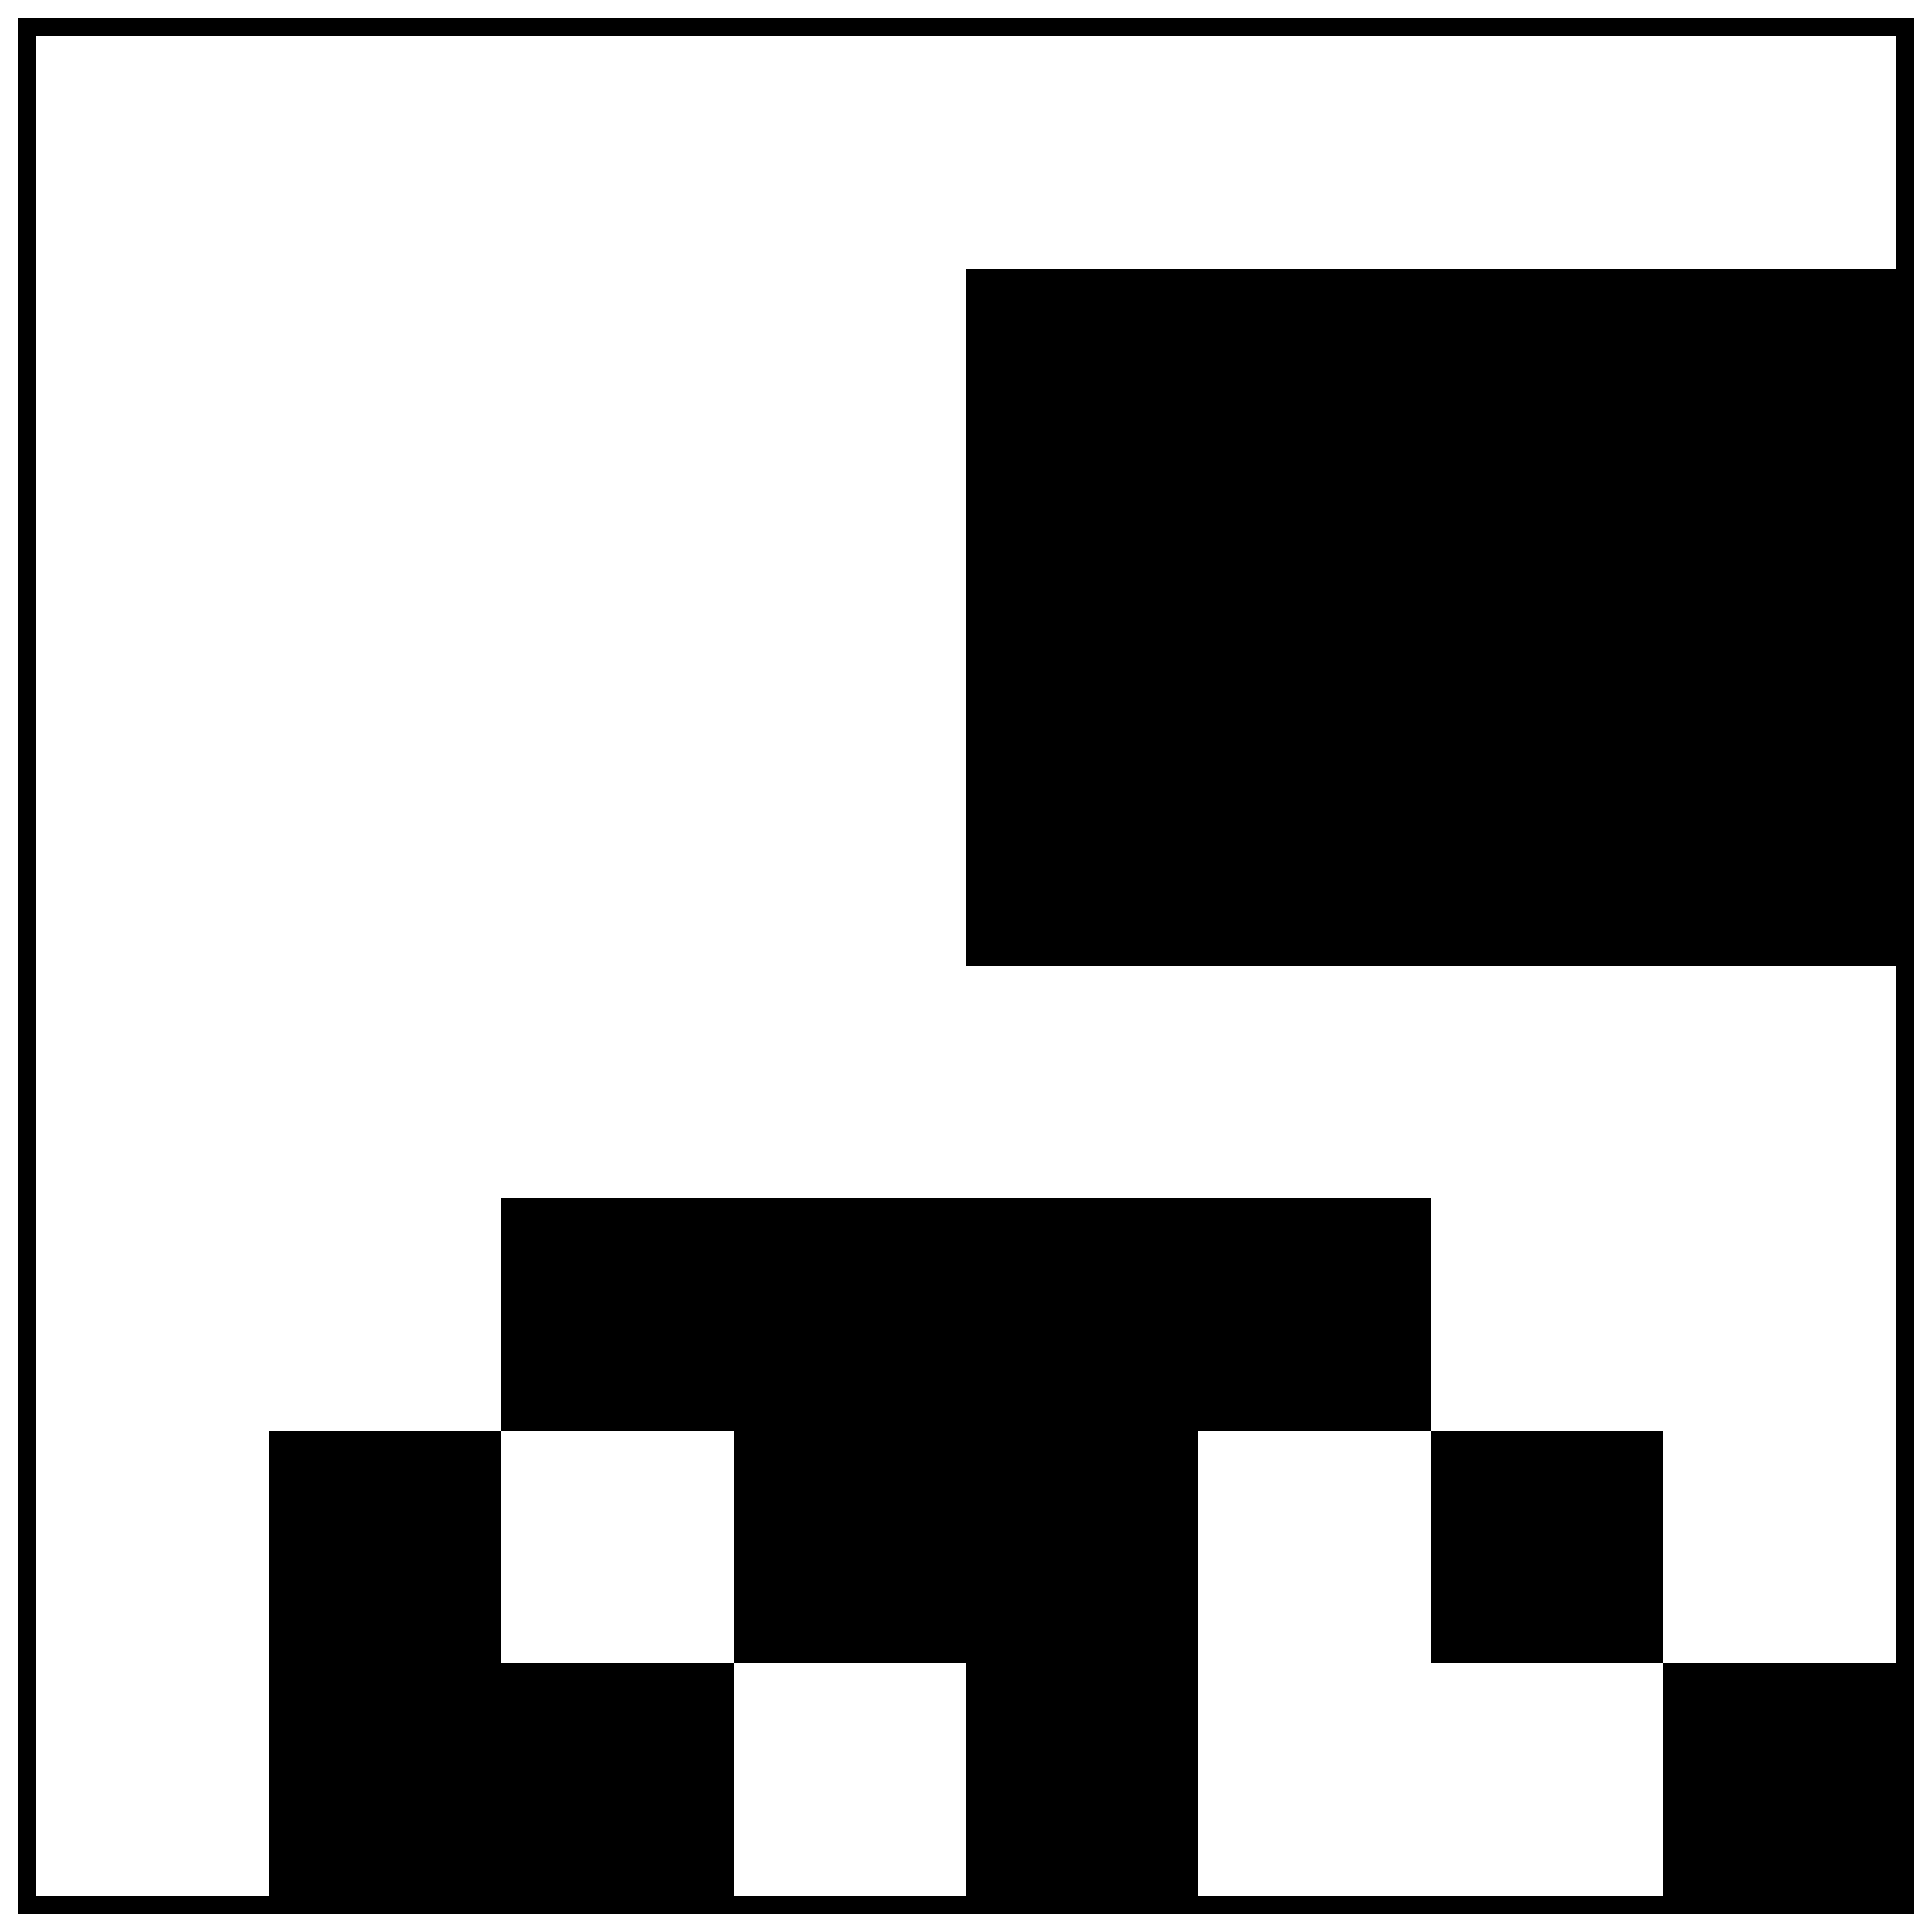
\includegraphics[width=0.25\textwidth]{m16.png}
\end{center}
\caption{Twisted cocycle for the Moufang loop $M$, white = $0$, black = $1$. The order of the row/colum labels is $000$, $100$, $010$, $110$, $001$, $101$, $011$, $111$. }\label{fig:cocycle for M}
\end{figure}


Notice in particular that the first four columns/rows correspond to the subgroup $U\subset V$ generated by $100$ and $010$, and that the restriction of $\mu$ to $U\times U$ is identically zero (i.e.\ white). 
This means that the \emph{restriction} $M\big|_U < M$ (the subloop of $M$ whose elements are mapped to $U$ by $M \to V$) is isomorphic to the direct product $\FF_2\times U$, and in particular a group.
\end{example}


\section{Codes and code loops.}

To describe the twisting function $f$ for our code loops, we need to know about some extra operations that exist on vector spaces over the field $\FF_2$. 
For $W$ an $n$-dimensional vector space over $\FF_2$ and vectors $v,w\in W$, there is a new vector $v\AND w \in W$ given by
\[
	v\AND w := (v_1w_1,\,v_2w_2,\,\ldots,\,v_nw_n).
\]
If we think of such vectors as binary strings, then this operation is bitwise AND. 
Note that if we take a code $\cC \subset (\FF_2)^n$, then $\cC$ is not guaranteed to be closed under this operation.
The other operation takes a vector $v\in W$ and returns its \emph{weight}: the sum, as an integer, of its entries: $|v| := v_1 + \cdots + v_n$. 
Equivalently, it is the number of nonzero entries in $v$.

The twisting function is then a combination of these two, namely $f(u,v,w) := |u\AND v\AND w|$.
However, as alluded to above, we are going to ask that further identities hold. 
For these identities to make sense we need to start with a code with the special property of being \emph{doubly even}.

\begin{definition}
A code $\cC \subset (\FF_2)^n$ is \emph{doubly even} if for every word $v\in \cC$, $|v|$ is divisible by 4. 
\end{definition}


\begin{example}\label{example:Hamming}
The \emph{Hamming (8,4) code} is the subspace of $(\FF_2)^8$ spanned by the rows of the matrix
\[
\begingroup % keep the change local
\setlength\arraycolsep{2pt}
\begin{pmatrix}
1&0&0&0&0&1&1&1\\
0&1&0&0&1&0&1&1\\
0&0&1&0&1&1&0&1\\
0&0&0&1&1&1&1&0
\end{pmatrix}
\endgroup
\]
and is doubly even.
\end{example}

A more substantial example is given by the Golay code.

\begin{example}\label{example:Golay}
The (extended binary) Golay code $\cG \subset (\FF_2)^{24}$ is the span of the following (row) vectors, denoted $b_1,\ldots,b_6$ (left) and $b_7,\ldots,b_{12}$ (right):
\[	
	 \begin{array}{c}
     000110000000010110100011 \\
     101001111101101111110001 \\
     000100000000100100111110 \\
     010000000010000110101101 \\
     000000000010010101010111 \\
     100000000000100111110001
     \end{array}
\qquad
    \begin{array}{c}
	 101001011100111001111111 \\
	 100000011100001001001100 \\
	 000001000000111001001110 \\
	 100000001000111000111000 \\
	 100000000100101000010111 \\
	 011011000001111011111111
	 \end{array}
\]
This basis is different to the more usual ones (e.g.\ \cite[Figure 3.4]{SPLAG}), which can be taken as the rows of a $12\times 24$ matrix whose left half is the $12\times 12$ identity matrix.
Our basis, however, allows us to demonstrate some interesting properties.
\end{example}

The inclusion/exclusion formula applied to counting nonzero entries allows us to show that, for all $v$ and $w$ in any doubly even code $\cC$,
\[
	|v+w| + |v\AND w| = |v| + |w| - |v\AND w|\,.
\]
In other words: $|v\AND w| = \frac12(|v| + |w| - |v+w|)$, which implies that $|v\AND w|$ is divisible by $2$.
Thus for words $v,w$ in a doubly even code, both $\frac14|v|$ and $\frac12|v\AND w|$ are integers.

\begin{definition}[Griess \cite{Griess}]
Let $\cC$ be a doubly even code. 
A \emph{code cocycle}\footnote{What we call a code cocycle, Griess actually calls a `factor set'. Given that a code cocycle is an example of a twisted cocycle, we prefer a name that indicates this.} is a function $\theta\colon \cC \times \cC \to \FF_2$ satisfying the identities
\begin{align}
& \theta(v,w)-\theta(u+v,w)+\theta(u,v+w)-\theta(u,v) =|u\AND v \AND w| \pmod 2 \label{eq: code cocycle 1}\\
& \theta(v,w)+\theta(w,v) = {}  \tfrac12|v\AND w| \pmod 2 \label{eq: code cocycle 2}\\
& \alpha(v,v) = {}  \tfrac14|v| \pmod 2\label{eq: code cocycle 3}
\end{align}
A \emph{code loop} is then a loop arising as $\FF_2\times_\theta \cC$ (up to isomorphism) for some code cocycle $\theta$.
\end{definition}

An example of a code cocycle appears in Figure~\ref{fig:cocycle for M}, so that the loop $M$ of Example~\ref{example:m16} is a code loop.

There is a notion of what it means for two twisted cocycles to be equivalent, and equivalent twisted cocycles give isomorphic loops.
As part of \cite[Theorem 10]{Griess}, Griess proves that all code cocycles for a given doubly even code are equivalent, and hence give isomorphic code loops. 

It is not obvious, on first consideration, that code cocycles even exist, or how many there are for a given doubly even code. 
However, Griess gave a proof that inductively constructs code cocycles, and counts how many arbitrary choices can be made along the way, proving that code cocycles do indeed exist.
The number of possible code cocycles quickly becomes fearsome: $2^{2^k-k-1}$, for $k=\dim \cC$ (\cite[Theorem 10]{Griess}).
For the $4$-dimensional Hamming code given above, this is $512$, but for the Golay code there are $2^{4083}$ possible code cocycles, a number with $1230$ digits in base $10$.
Even though there are many code cocycles, finding even one by brute force is completely infeasible.
The set of all possible functions $\cC\times \cC \to \FF_2$ has $2^{k^2}$ elements; for the Golay code ($k=12$) this number is astronomical.




\section{Griess's algorithm and its output.}

The algorithm that Griess describes in the proof of \cite[Theorem 10]{Griess} to construct code cocycles for a code $\cC$ takes as input an ordered  basis $\{b_0,\ldots,b_{k-1}\}$ for $\cC$. 
The code cocycle is then built up inductively over larger and larger subspaces $V_i = \Span\{b_1,\ldots,b_i\}$.%, at each stage applying the identities to define the growing code cocycle on a larger domain.

However, the description by Griess is more of an outline, using steps like `determine the cocycle on such-and-such subset using identity X', where X refers to one of (\ref{eq: code cocycle 1}), (\ref{eq: code cocycle 2}), (\ref{eq: code cocycle 3}), or corollaries of these. We have reconstructed the process in detail in Algorithm~\ref{Griess algo}.

\begin{algorithm}[b]
\small
\caption{Reverse engineered from proof of \cite[Theorem 10]{Griess}.}\label{Griess algo}
\SetAlgoLined
\DontPrintSemicolon
\KwData{Basis $B = \{b_0,b_1,\ldots,b_{k-1}\}$ for the code $\cC$}
\KwResult{Code cocycle $\theta\colon \cC\times \cC\to \FF_2$, encoded as a square array of elements from $\FF_2$, with rows and columns indexed by $\cC$ }
\;
\tcp{Initialise} 
\ForAll{$c_1,c_2 \in C$}{
$\theta(c_1,c_2) \leftarrow 0$\;
}

$\theta(b_0,b_0) \leftarrow \tfrac14\left|b_0\right|$\;
\;
\ForAll{$1\leq i\leq \Length(B)$}{
	Define $V_i :=\Span\{b_0,\ldots,b_{i-1}\}$\;
	\tcp{(D1) define theta on \{bi\} x Vi then deduce on Vi x \{bi\}}
	\ForAll{$v\in V_i$}{
		\eIf{$v\neq0$}{
			$\theta(b_i,v) \leftarrow \text{random}$ \tcp*{In practice, random = 0}
			$\theta(v,b_i) \leftarrow \tfrac12\left|v\And b_i\right|+\theta(b_i,v)$\;
		}
		{
			\tcp{$\theta(b_i,v)$ is already set to 0}
			$\theta(v,b_i)\leftarrow \tfrac12\left|v\And b_i\right|$\;
		}
	}
	\tcp{(D2) deduce theta on \{bi\} x Wi and Wi x \{bi\}}
	\ForAll{$v\in V_i$}{
		$\theta(b_i,b_i\Plus v) \leftarrow \tfrac14\left|b_i\right| + \theta(b_i,v)$\;
		$\theta(b_i\Plus v,b_i) \leftarrow \tfrac12\left|b_i\And (b_i\Plus v)\right| + \tfrac14\left|b_i\right| + \theta(b_i,v)$\;
	}
	\tcp{(D3) deduce theta on Wi x Wi}
	\ForAll{$v_1\in V_i$}{
		\ForAll{$v_2\in V_i$}{
			$w\leftarrow b_i \Plus v_2$\;
			$a\leftarrow \theta(v_1,b_i)$\;
			$b\leftarrow \theta(v_1,b_i\Plus w)$\;
			$c\leftarrow \theta(w,b_i)$\;
			$r \leftarrow \tfrac12\left|v_1\And w\right| + a + b + c$\;
			$\theta(w,b_i\Plus v_1) \leftarrow r$
		}
	}
	\tcp{(D4) deduce theta on Wi x Vi and Vi x Wi}
	\ForAll{$v_1\in V_i$}{
		\ForAll{$v_2\in V_i$}{
			$w\leftarrow b_i \Plus v_2$\;
			$a\leftarrow \theta(w,v_1\Plus w)$\;
			$\theta(w,v_1) \leftarrow \tfrac14\left|w\right| + a$\;
			$\theta(v_1,w) \leftarrow \tfrac12\left|v_1\And w\right| + \tfrac14\left|w\right| + a$\;
		}
	}
}
\end{algorithm}

We implemented Algorithm~\ref{Griess algo} in the language Go \cite{RN_GH}, together with diagnostic tests, for instance to verify the Moufang property.
The output of the algorithm is the code cocycle, encoded as a matrix of ones and zeroes, and can be displayed as an array of black and white pixels.
For the Golay code this image consists of slightly over 16 million pixels.

As a combinatorial object, the code cocycle $\theta\colon \cG \times \cG\to \FF_2$ constructed from Algorithm~\ref{Griess algo} using the basis in Example~\ref{example:Golay} is too large and unwieldy to examine for any interesting structure. 
Moreover, to calculate with the Parker loop $\cP := \FF_2\times_\theta \cG$ one needs to know all 16 million or so values of $\theta$.
It is thus desirable to have a method that will calculate values of $\theta$ by a method shorter than Algorithm~\ref{Griess algo}.

\begin{lemma}\label{lemma:formula lemma}
Let $\cC$ be a doubly even code, $\theta$ a code cocycle on it, and $\cC = V\oplus W$ a decomposition into complementary subspaces.
Then for $v_1,v_2\in V$ and $w_1,w_2\in W$,
\begin{align}\label{eq:theformula}
	\theta(v_1\Plus w_1,v_2\Plus w_2)	
		& = \theta(v_1,v_2)  + \theta(w_1,w_2) + \theta(v_1,w_1) \\
		&+ \theta(w_2,v_2) + \theta(v_1\Plus v_2,w_1\Plus w_2) \nonumber \\
							& + \tfrac12|v_2\And(w_1\Plus w_2)| + |v_1\And v_2 \And (w_1\Plus w_2)| \nonumber \\
							&+|w_1\And w_2 \And v_2| + \left|v_1\And w_1 \And (v_2 \Plus  w_2)\right| \pmod 2\,. \nonumber
\end{align}
\end{lemma}

\begin{proof}
We apply the identity (\ref{eq: code cocycle 1}) three times and then the identity (\ref{eq: code cocycle 2}) once:
\begin{align*}
\begin{split}
	\theta(v_1+w_1,v_2+w_2) =&\ \theta(v_1,w_1) + \theta(v_1,v_2+w_1+w_2) + \theta(w_1,v_2+w_2) \\
	&+ |v_1\AND w_1\AND(v_2+w_2)| 
\end{split}\\
\begin{split}
	 =&\ \theta(v_1,w_1) + \big\{ \theta(v_1,v_2) + \theta(v_1+v_2,w_1+w_2)) \\ 
	 & + \theta(v_2,w_1+w_2) + |v_1\AND v_2 \AND (w_1+w_2)| \big\} \\
	 & + \big\{\theta(w_1,w_2) + \theta(w_1+w_2,v_2) + \theta(w_2,v_2) + |w_1\AND w_2\AND v_2| \big\} \\
	 & + |v_1\AND w_1\AND(v_2+w_2)| 
\end{split}\\
\begin{split}
	 =&\ \theta(v_1,w_1) + \big\{ \theta(v_1,v_2) + \theta(v_1+v_2,w_1+w_2)) \\ 
	 & +  |v_1\AND v_2 \AND (w_1+w_2)| \big\} \\
	 & + \big\{\theta(w_1,w_2) + \theta(w_2,v_2) + |w_1\AND w_2\AND v_2| \big\} \\
	 & + |v_1\AND w_1\AND(v_2+w_2)| + \tfrac12|v_2\AND (w_1+w_2)| \qedhere
\end{split}
\end{align*}
\end{proof}

Observe that in Lemma~\ref{lemma:formula lemma}, on the right hand side of (\ref{eq:theformula}), the code cocycle $\theta$ is only ever evaluated on vectors from the subset $V \cup W \subset \cC$.
This means we can throw away the rest of the array and still reconstruct arbitrary values of $\theta$ using (\ref{eq:theformula}).
If we assume that $\cC$ is $2k$-dimensional, and that $V$ and $W$ are both $k$-dimensional, then the domain of the restricted $\theta$ has $(2^k+2^k - 1)^2 = 2^{2(k+1)} - 2^{k+2} + 1 = O((2^k)^2)$ elements. 
Compared to the full domain of $\theta$, which has $2^{2k}\times 2^{2k} = (2^k)^4$ elements, this is roughly a square-root saving.

And, now it should be clear why the Golay code basis in Example~\ref{example:Golay} was partitioned into two lists of six vectors: we can reconstruct all $16,777,216$ values of the resulting code cycle $\theta$, and hence the Parker loop multiplication, from a mere $2^{14} - 2^8 + 1 = 16,129$ values.
The span of the left column of vectors in Example~\ref{example:Golay} is the subspace $V\subset \cG$, and the span of the right column of vectors is $W\subset \cG$.

The top left quadrant of Figure~\ref{fig:Parker cocycle} then contains to the restriction of $\theta$ to $V\times V$, and the bottom right quadrant the restriction to $W\times W$. 
The off-diagonal quadrants contain the values of $\theta$ restricted to $V\times W$ and $W\times V$.

\begin{figure}[ht]
\begin{center}
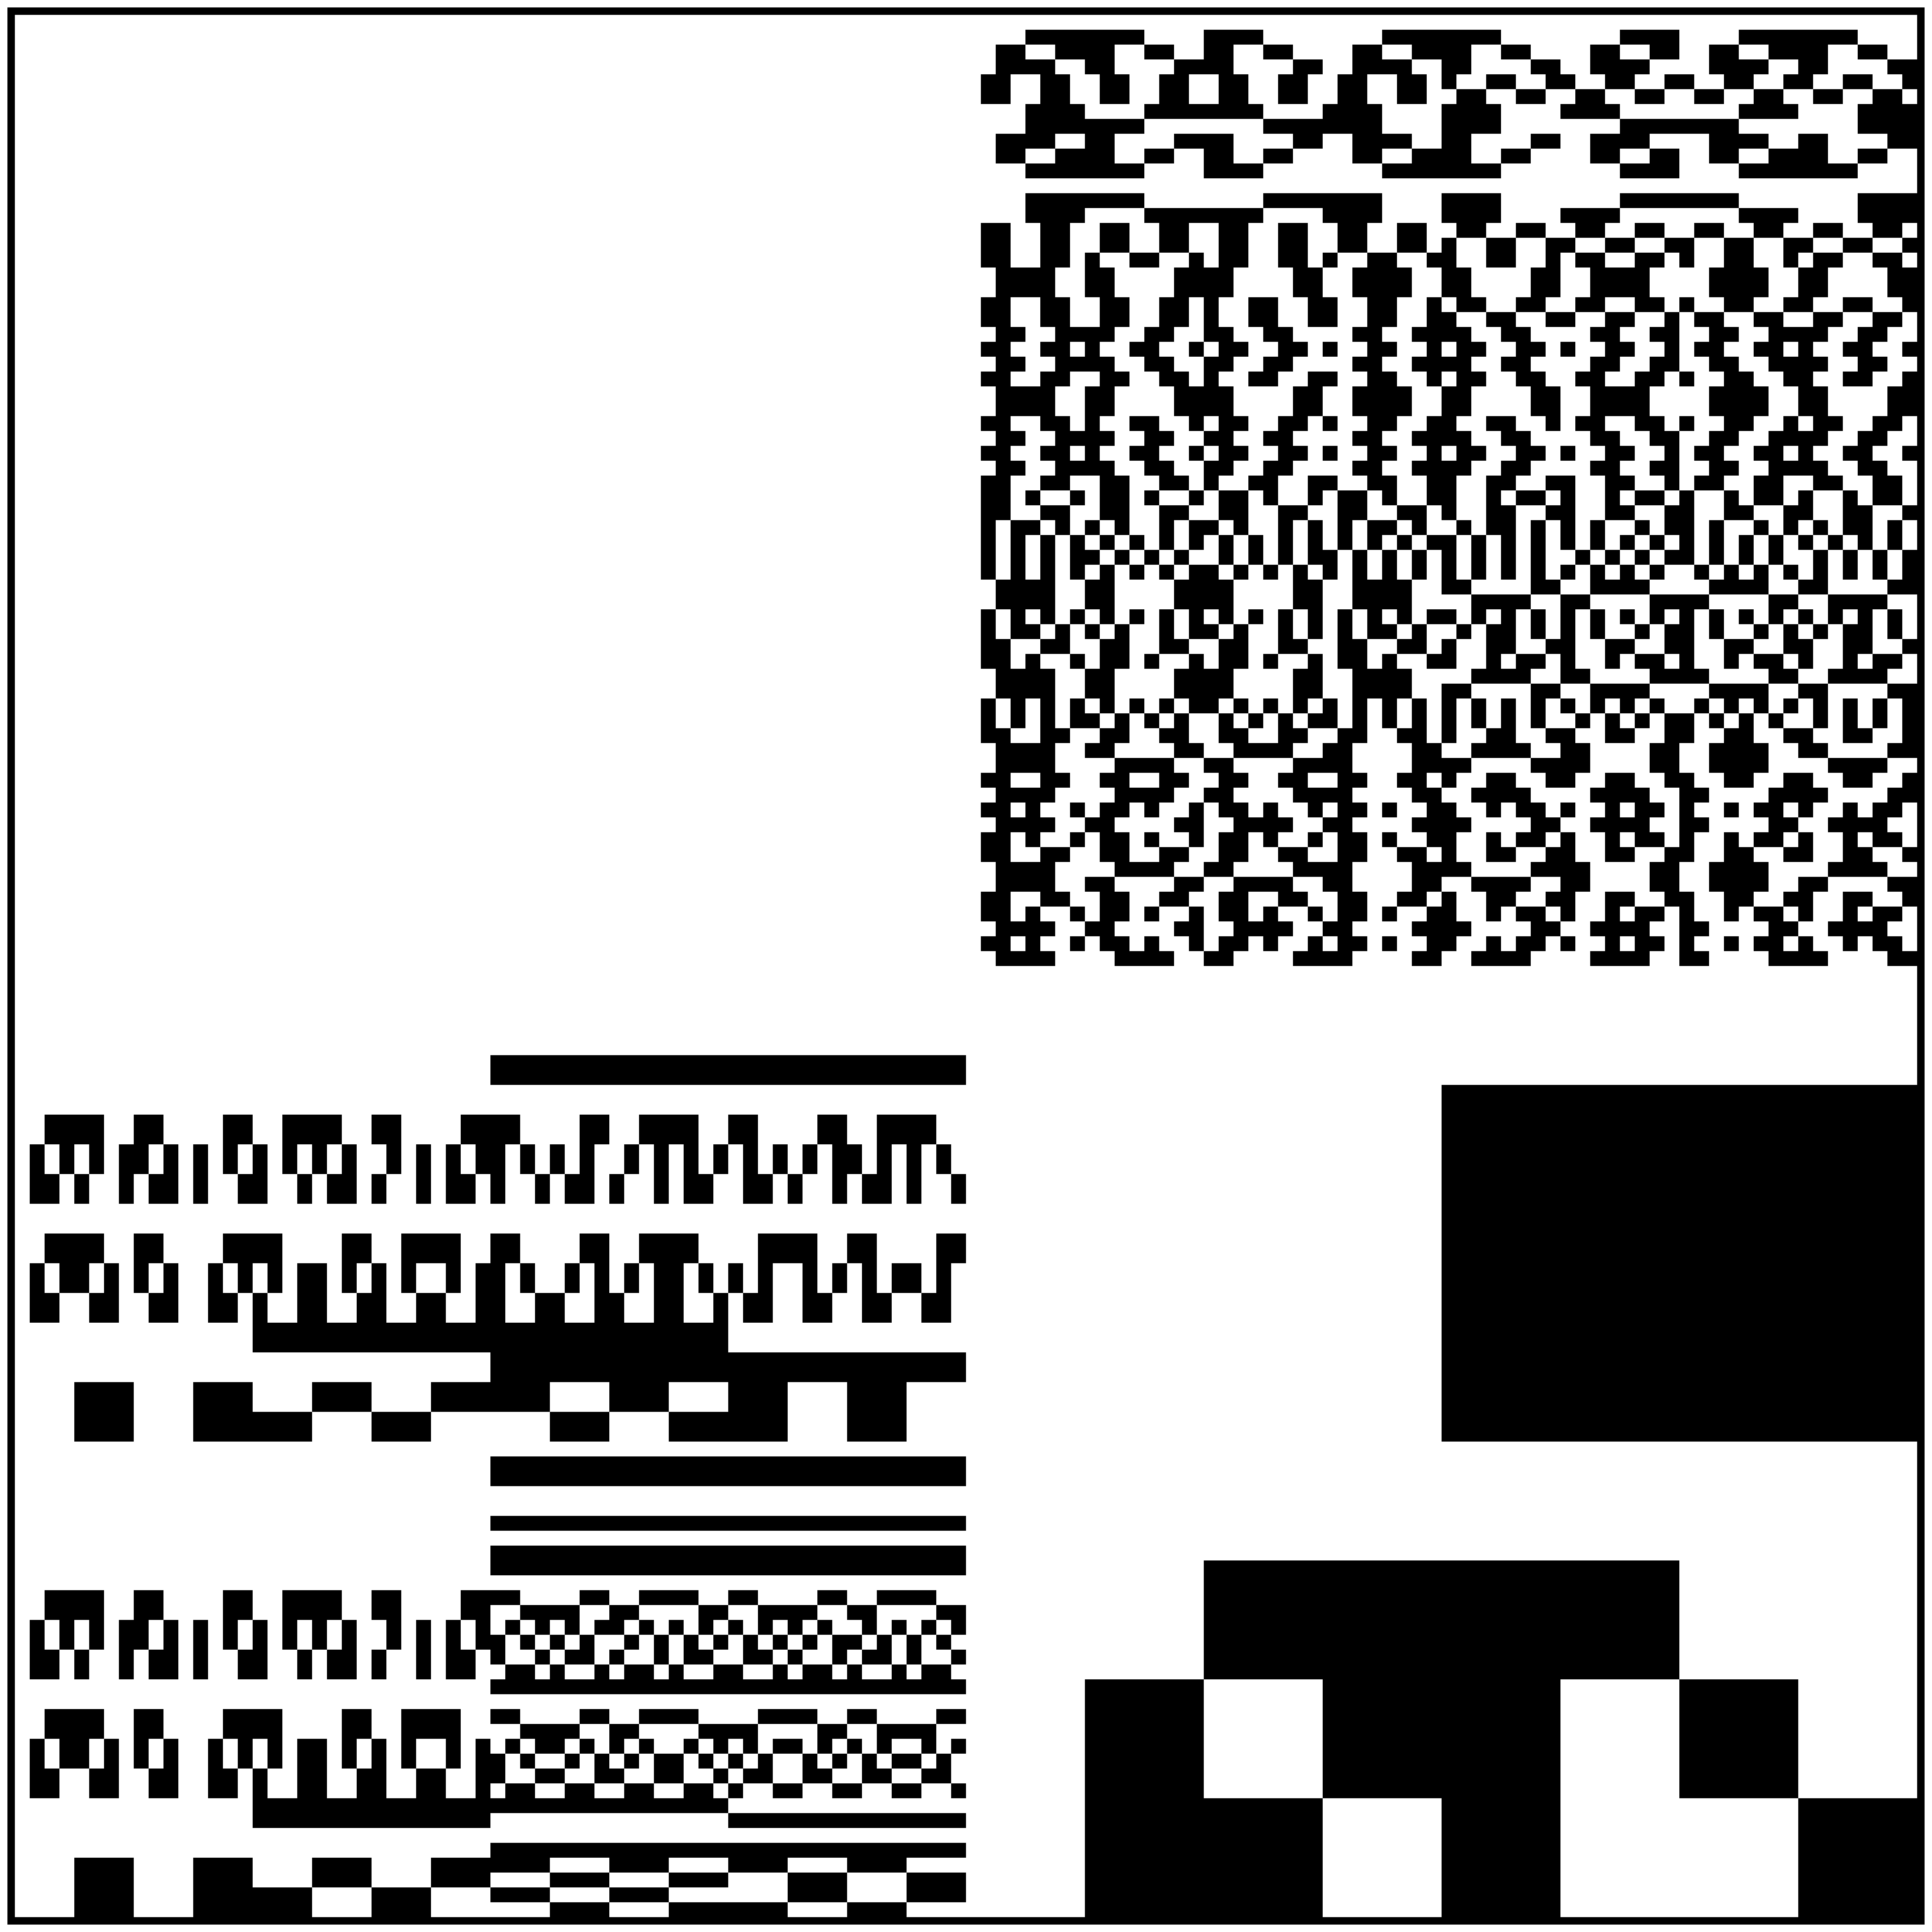
\includegraphics[width=0.8\textwidth]{alpha_awesum.png}
\end{center}
\caption{The restriction of the Parker loop code cocycle $\theta$ to $(V\cup W)^2$. A machine-readable version is available in \cite{RN_GH} or as an arXiv ancillary file. The order of the row/column labels is $\underline{0},b_1,b_2,b_1+b_2,b_3,\ldots, b_1+\cdots +b_6$, $b_7,b_8,b_7+b_8,\ldots,b_7+\cdots + b_{12}$.}
\label{fig:Parker cocycle}
\end{figure}

From Figure~\ref{fig:Parker cocycle} we can immediately see that the restriction of the Parker loop $\cP\big|_V$ reduces to a direct product, as $\theta\big|_{V\times V}$ is identically zero. 
Moreover, the restriction of $\cP\big|_W$ is the direct product $(\FF_2)^3 \times M$, where $M$ is the Moufang loop from Example~\ref{example:m16}.
This is because what was a single pixel in Figure~\ref{fig:cocycle for M} is now an $8\times 8$ block of pixels in Figure~\ref{fig:Parker cocycle}.

\section{Discussion and comparison}

The Parker loop $\cP$ is a sporadic object that has spawned a small industry trying to understand and construct code loops in general, as a class of Moufang loops that are fairly easy to describe.

Aside from the description by Griess using code cocycles, there was an unpublished description by Parker, an unpublished thesis \cite{Johnson}, characterisations as loops with specified commutators and associators \cite{CheinGoodaire}, an iterative construction using centrally twisted products \cite{Hsu}, and a construction using groups with triality \cite{Nagy}. 
The LOOPS library \cite{LOOPS} for software package GAP \cite{GAP4} contains all the code loops of order $64$ and below, although ``the package is intended primarily for quasigroups and loops of small order, say up to $1000$''.
Even the more recent \cite{OBrien_Vojtechovsky}, which classifies code loops up to order $512$ in order to add them to the LOOPS package, falls short of the Parker loop's $8192$ elements; the authors say ``our work suggests that it will be difficult to extend the classification of code loops beyond order $512$''.
In principle, there is nothing stopping the construction of $\cP$ in LOOPS, but it will essentially be stored as a multiplication table, which would comprise $67,108,864$ entries, each of which is a $13$-bit element label.
The paper \cite{Morier-Genoud_Ovsienko} describes an algebraic formula for a code cocycle that will build the Parker loop, as a combination of the recipe in the proof of Proposition~6.6 and the generating function in Proposition~9.2.
This formula is a polynomial with $330$ cubic terms and $12$ quadratic terms in $24$ variables, being coefficients of basis vectors of $\cG$. 
To compare, combined with the small amount of data in Figure~\ref{fig:Parker cocycle} together with a labelling of rows/columns by words of the Golay code, Lemma~\ref{lemma:formula lemma} only requires 9 terms, of which four are cubic and the rest come from the $16,129$ stored values of $\theta$.
Large-scale computation in large code loops requires optimising the loop product, and we have found a space/time trade-off that must surely approach the more effective end of the spectrum.

In addition to computational savings, the ability to visually explore the structure of code loops during experimentation more generally seems a novel advance---the recognition of $(\FF_2)^3\times M$ inside $\cP$ was purely by inspection of the picture of the code cocyle then consulting the small list of Moufang loops of small order \cite{Chein}.
Discovery of the basis in Example~\ref{example:Golay} was by walking through the spaces of bases of subcodes and working with the heuristic that more regularity in the appearance of the code cocycle is better.
Additionally, our code flagged when subloops thus considered were in fact associative, and hence a group, leading to the discovery of the relatively large elementary subgroups $(\FF_2)^7 < \cP$ and $(\FF_2)^6 < (\FF_2)^3\times M < \cP$. 

Finally, one can also remark that because of the identity (\ref{eq: code cocycle 2}), one can reconstruct the top right quadrant of Figure~\ref{fig:Parker cocycle} from the bottom left quadrant, and vice versa. 
Thus one can describe the Parker loop as being generated by the subloops $(\FF)^7$ and $(\FF_2)^3\times M$, with relations coming from the information contained in the bottom left quadrant of Figure~\ref{fig:Parker cocycle}, and the formulas (\ref{eq: code cocycle 2}) and (\ref{eq:theformula}).
The regularity in that bottom left quadrant is intriguing, and perhaps indicative of further simplifications; this will be left to future work.





\begin{acknowledgment}{Acknowledgment.}
DMR is supported by the Australian Research Council's Discovery Projects scheme, (project number DP180100383), funded by the Australian Government.
\end{acknowledgment}

\begin{thebibliography}{1}
\bibitem{Chein} Orin Chein, Moufang Loops of Small Order.\ I, \emph{Trans.\ Am. Math. Soc.} \textbf{188} (1974) 31--51.

\bibitem{CheinGoodaire} Orin Chein and Edgar G.\ Goodaire, Moufang loops with a unique nonidentity commutator (associator, square), \emph{J.\ Algebra} \textbf{130} (1990) 369--384.

\bibitem{Conway} John H.\ Conway, A simple construction for the Fischer--Griess monster group, \emph{Invent.\ math.} \textbf{79} (1985) 513--540.

\bibitem{SPLAG} John H.\ Conway and Neil Sloane, Sphere packings, lattices and groups. Third Edition. Grundlehren der Mathematischen Wissenschaften \textbf{290} Springer-Verlag, New York, 1999.

\bibitem{GAP4} The GAP~Group, \emph{GAP -- Groups, Algorithms, and Programming, Version 4.10.0} (2018) \url{https://www.gap-system.org}.

\bibitem{Griess} Robert L.\ Griess Jr., Code loops, \emph{J.\ Algebra} \textbf{100} (1986) 224--234.

\bibitem{Hsu} Tim Hsu, Explicit constructions of code loops as centrally twisted products, \emph{Math.\ Proc.\ Cam.\ Phil.\ Soc.} \textbf{128} (2000) 223--232.

\bibitem{Johnson} Peter Johnson, Gamma spaces and loops of nilpotence class two, PhD thesis, University of Illinois at Chicago, 1988.

\bibitem{LOOPS} G\'abor P.\ Nagy and Petr Vojt\v{e}chovsk\'{y}, LOOPS: Package for GAP, Version 3.4.0. \url{https://www.cs.du.edu/~petr/loops/}, 2017.

\bibitem{Morier-Genoud_Ovsienko} Sophie Morier-Genoud and Valentin Ovsienko, A series of algebras generalizing the octonions and Hurwitz-Radon identity, \emph{Commun. Math. Phys.} \textbf{306} (2011) 83--118, arXiv:1003.0429

\bibitem{Moufang} Ruth Moufang, Zur Struktur von Alternativk\"orpern \emph{Math. Ann.} \textbf{110} (1935) 416--430. doi:10.1007/bf01448037

\bibitem{RN_GH} Ben Nagy and David Michael Roberts, \texttt{codeloops}, GitHub repository, (2019) \url{https://github.com/bnagy/codeloops}

\bibitem{Nagy} G\'abor P.\ Nagy, Direct construction of code loops, \emph{Discrete Mathematics} \textbf{308} (2008) 5349--5357.

\bibitem{OBrien_Vojtechovsky} Eamonn A.\ O'Brien and and Petr Vojt\v{e}chovsk\'{y}, Code loops in dimension at most 8, \emph{J.\ Algebra} \textbf{473} (2017) 607--626, arXiv:1712.06524.

% \bibitem{Thompson} Thomas M.\ Thompson, From Error Correcting Codes through Sphere Packings to Simple Groups. Carus Mathematical Monographs. \textbf{21}. Mathematical Association of America, Washington, DC, 1983. 
\end{thebibliography}

\begin{biog}
\item[Ben Nagy] is an MPhil.\ candidate at the University of Adelaide, researching computational stylistics for Latin Poetry.
\begin{affil}
Department of Classics, Archaeology \& Ancient History, The University of Adelaide\\
benjamin.nagy@adelaide.edu.au
\end{affil}

\item[David Michael Roberts] is a mathematician specialising in category theory, geometry and a hodge-podge of other random topics.
\begin{affil}
School of Mathematical Sciences, The University of Adelaide\\
david.roberts@adelaide.edu.au
\end{affil}
\end{biog}
\vfill\eject

\end{document}